\setcounter{equation}{0}
\chapter{Model}

We use the simplified rotation model developed by \cite{Garavito14} in which a rotating galaxy is modeled as a solid rotating sphere, with a homogeneous mixture of hydrogen and dust. There is also the radial expanding velocity. Photons are initially at the center of the sphere. These two velocities are added by components as follows. The equations governing this movement in which the axis of rotation is defined to be align with the $z$-axis are: 

\begin{equation}
v_{x}=\frac{x}{R}v_{\rm out}-\frac{y}{R}v_{\rm rot}, \label{subeq1}
\end{equation}

\begin{equation}
v_{y}=\frac{y}{R}v_{\rm out}+\frac{x}{R}v_{\rm rot}, \label{subeq2}
\end{equation}

\begin{equation}
v_{z}=\frac{z}{R}v_{\rm out}, \label{subeq3}
\end{equation}

Where $R$ is the radius of the sphere. The minus/plus sign in the $x$/$y$-component of the rotation velocity part indicates the direction of rotation. In this case we take the angular velocity in the same direction as the $\hat{k}$ unit vector. \\

Now, we'll describe the radiative transfer process that is simulated by the code. Each photon is emitted with the natural \lya frequency from the center of the galaxy. The individual scattering of the emitted photon is tracked through a 3D distribution of neutral Hydrogen. The frequency of the photon and its direction of propagation change at every encounter due to the peculiar velocities of the Hydrogen absorbing it and re-emitting it. Once the photon escape the galaxy, its final values are stored: position, direction of propagation, frequency and number of scatterings. For each simulation a histogram of this final frequencies is created and it represents the \lya associated to the initial configuration.\\

We express a photon's frequency in terms of the dimensionless variable:

\begin{equation}
x\equiv (\nu -\nu_a)/\Delta\nu_{\rm D}
\end{equation} 

Where $\nu_{\rm \alpha}=2.46\times 10^{15}$ Hz is the Ly$\alpha$ resonance frequency,  $\Delta\nu_{\rm D} \equiv \nu_{\alpha}\sqrt{2kT/m_pc^2}\equiv \nu_av_{\rm th}/c $ is the Doppler broadening of the line which depends on the neutral gas temperature $T$ or equivalently the thermal velocity $v_{\rm th}$ of the atoms. For the temperature $T=10^4$K used in our radiative transfer calculations the thermal velocity is $v_{\rm th}=12.8$\kms.   \\

\section{Galaxy Parameters}

Our aim is to provide a realistic baseline to compare against observations of LAEs at $z\sim 3$. It has been found by analysis of the abundance and angular correlation function that LAEs reside in DM halos of masses in the range $10^{10}-10^{11}$\Msun \cite{WalkerSoler2012}. This mass range corresponds to maximum circular velocities in the range $60-125$\kms and a median halo scale radius of $15$kpc. \footnote{These results were found using the  N-body data available in \url{www.cosmosim.org}}. \\

These galaxies have gas fractions close to $20\%$ (\cite{Narayanan2012}). We approximate that the hydrogen content is $20\%$ the total baryonic content from the cosmological baryon to dark matter  abundances $\Omega_b/\Omega_{dm}=0.1825$ (\cite{Planck2015}), multiplied by a primordial Hydrogen fraction of $0.75$. All these considerations gives us hydrogen masses in the range $2.7\times 10^{8}-2.7\times 10^{9}$\Msun.\\

These choices give us a range for the number density of Hydrogen atoms of $4\times10^{-4}-4\times 10^{-3}$ atoms cm$^{-3}$. With a Lyman-$\alpha$ cross section at the line center of $\sigma_{H}=1.0\times 10^{-14}$ cm$^{2}$ we finally obtain that the optical depth from the cloud's center  should be in the range $\tau_{\rm H}=2 \times 10^{5} - 2 \times 10^{6}$.  \\

In order to be able to tell the influence of the rotation and outflows velocities in the \lya line morphology, a mapping of them is made without concerning of their physical meaning at first, this constitutes the 1st run. In the second run the interesting ranges are identified and narrowed. In the 3rd and last run, the final physical and relevant combinations are made. \\

All of the selected values with its corresponding run are registered in Tab. \ref{tab:runs}. The way to read it is: for the $i^{th}$ run, all of the permutations of \tauh, \vrot and \vout are run.

\begin{table}[htbp]
	\centering
	\begin{tabular}{|c|c|c|c|}
		\hline
		\textbf{RUN} & \bv{1^{st}} & \bv{2^{nd}} & \bv{3^{rd}} \\
		\hline
		\tauh & 5, 6, 7 & 5, 6, 7 & 5, 6 \\
		\hline
		\vrot (\kms) & 0, 100, 200 ,300 & 50, 100 & 50, 100 \\
		\hline
		\vout (\kms) & 100, 200, 300 & 25, 50, 75 & 5, 10, 15, 20 \\
		\hline
	\end{tabular}%
	\caption{\textbf{Combinations of values in each run.}}
	\label{tab:runs}%
\end{table}%

Is important to note that if we stand next to the galaxy, not all of the photons emitted are going to be observed because some will have directions that could never reach our position. For this reason, it is very important to define viewing angle so that only photons that escape within that range are counted in the spectrum. As seen in Fig. \ref{fig:viewing_angle_sketch}, only the photons with escaping direction angle $\theta$ respect to the rotation axis that belongs to the range $[\theta_{min}-\theta_{max}]$ will be reach the observer. 

\begin{figure}[h!]
	\begin{center}
		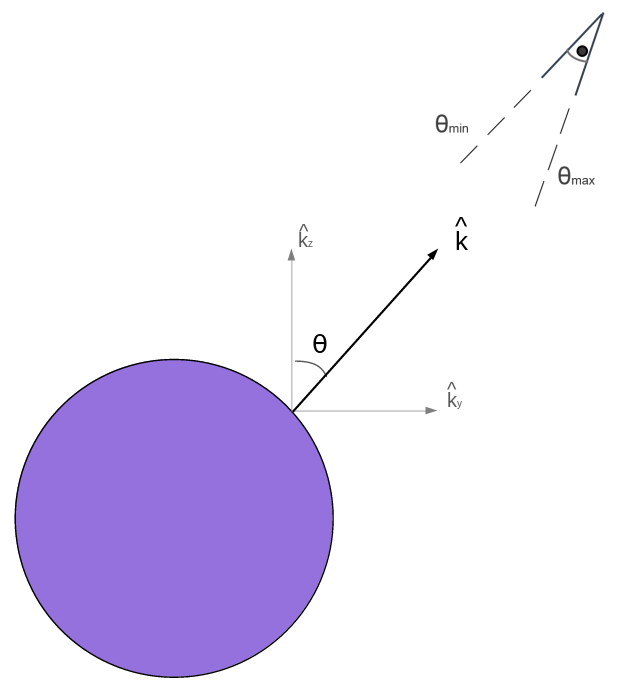
\includegraphics[width=0.6\textwidth]{./figures/chapter2/viewing_angle_sketch}
	\end{center}
	\caption{\textbf{Viewing Angle Sketch:} The galaxy is in the $y-z$ plane perspective and the eye is located at an specific viewing angle of the sphere. Only photons with a direction that enters in his range of vision can enter to the result.
		\label{fig:viewing_angle_sketch}}
\end{figure}

This creates 2 new parameters, the azimuthal angle and the polar angle. However, the galaxy's movement is symmetrical respect to its rotation axis, which implies that the resulting spectrum will not vary depending on the azimuthal angle. This lets us then take all of the photons with azimuthal viewing angle from $0$ to $2\pi$ for each selected polar range, which we will do for statistical reasons. Regarding the polar angle, we will take spectra from 9 different ranges from $0$ to $\pi$ that are uniform in $\cos(\theta)$ and analyze the influence of this effect as well. All of these results will be seen in the next chapter. 